%%%%%%%%%%%%%%%%%%%%%%%%%%%%%%%%%%%%%%%%%
% Texas A&M University Physics Template
% This template has been downloaded from:
% http://www.LaTeXTemplates.com
%
% Modified by Joe Becker
%
% License:
% CC BY-NC-SA 3.0 (http://creativecommons.org/licenses/by-nc-sa/3.0/)
%
%%%%%%%%%%%%%%%%%%%%%%%%%%%%%%%%%%%%%%%%%

%----------------------------------------------------------------------------------------
%	PACKAGES AND THEMES
%----------------------------------------------------------------------------------------

\documentclass{beamer}

\mode<presentation> 

\usetheme{Madrid}
\usecolortheme{dolphin}
\usefonttheme{professionalfonts}

\setbeamertemplate{navigation symbols}{} 

\setbeamertemplate{footline}
{
\leavevmode%
\hbox{%
    \begin{beamercolorbox}[wd=.333333\paperwidth,ht=2.25ex,dp=1ex,center]{section in head/foot}%
        \usebeamerfont{author in head/foot}\insertshortauthor \ {(\insertshortinstitute)}
    \end{beamercolorbox}%
    \begin{beamercolorbox}[wd=.333333\paperwidth,ht=2.25ex,dp=1ex,center]{section in head/foot}%
        \usebeamerfont{title in head/foot}\insertshorttitle
    \end{beamercolorbox}%
    \begin{beamercolorbox}[wd=.333333\paperwidth,ht=2.25ex,dp=1ex,right]{section in head/foot}%
        \usebeamerfont{date in head/foot}\insertshortdate{}\hspace*{2em}
    \end{beamercolorbox}}%
    \vskip0pt%
}

\setbeamertemplate{frametitle}
{
    \begin{beamercolorbox}[sep=0.3cm,ht=1.8em,wd=\paperwidth]{frametitle}
        \vbox{}\vskip-0.0ex%
        \strut\insertframetitle\strut
        \hfill
        \vskip-2.8ex%
    \end{beamercolorbox}
}

\definecolor{maroon}{RGB}{25,25,112}

\setbeamercolor{title}{bg=maroon, fg=white}
\setbeamercolor{block title}{bg=maroon, fg=white}
\setbeamercolor{block body}{bg=maroon!05, fg=black}
\setbeamercolor{frametitle}{fg=maroon, bg=white}
\setbeamercolor{item}{fg=maroon}
\setbeamercolor{section in head/foot}{bg=maroon, fg=white}


\usepackage{graphicx}
\usepackage{booktabs}
\usepackage{textpos} 
\usepackage{media9}
\usepackage{natbib}


%----------------------------------------------------------------------------------------
%	TITLE PAGE
%----------------------------------------------------------------------------------------

\title[OSA News]{Cosmic Bell Test: Measurement Settings from Milky Way Stars}

\author[J. Becker]{Joe Becker}

\institute[Texas A\&M]{Texas A\&M Department of Physics and Astronomy

\medskip
\textit{jbecker@physics.tamu.edu} 
}

\date{February 16, 2017} 

\titlegraphic{
\includegraphics[height=2.5cm]{Images/TAMU_logo.png}}

%----------------------------------------------------------------------------------------
% PRESENTATION SLIDES
%----------------------------------------------------------------------------------------

\begin{document}
\setbeamertemplate{items}[circle]

\begin{frame}
\titlepage 
\end{frame}

\begin{frame}{Local Realism}
    \begin{center}
    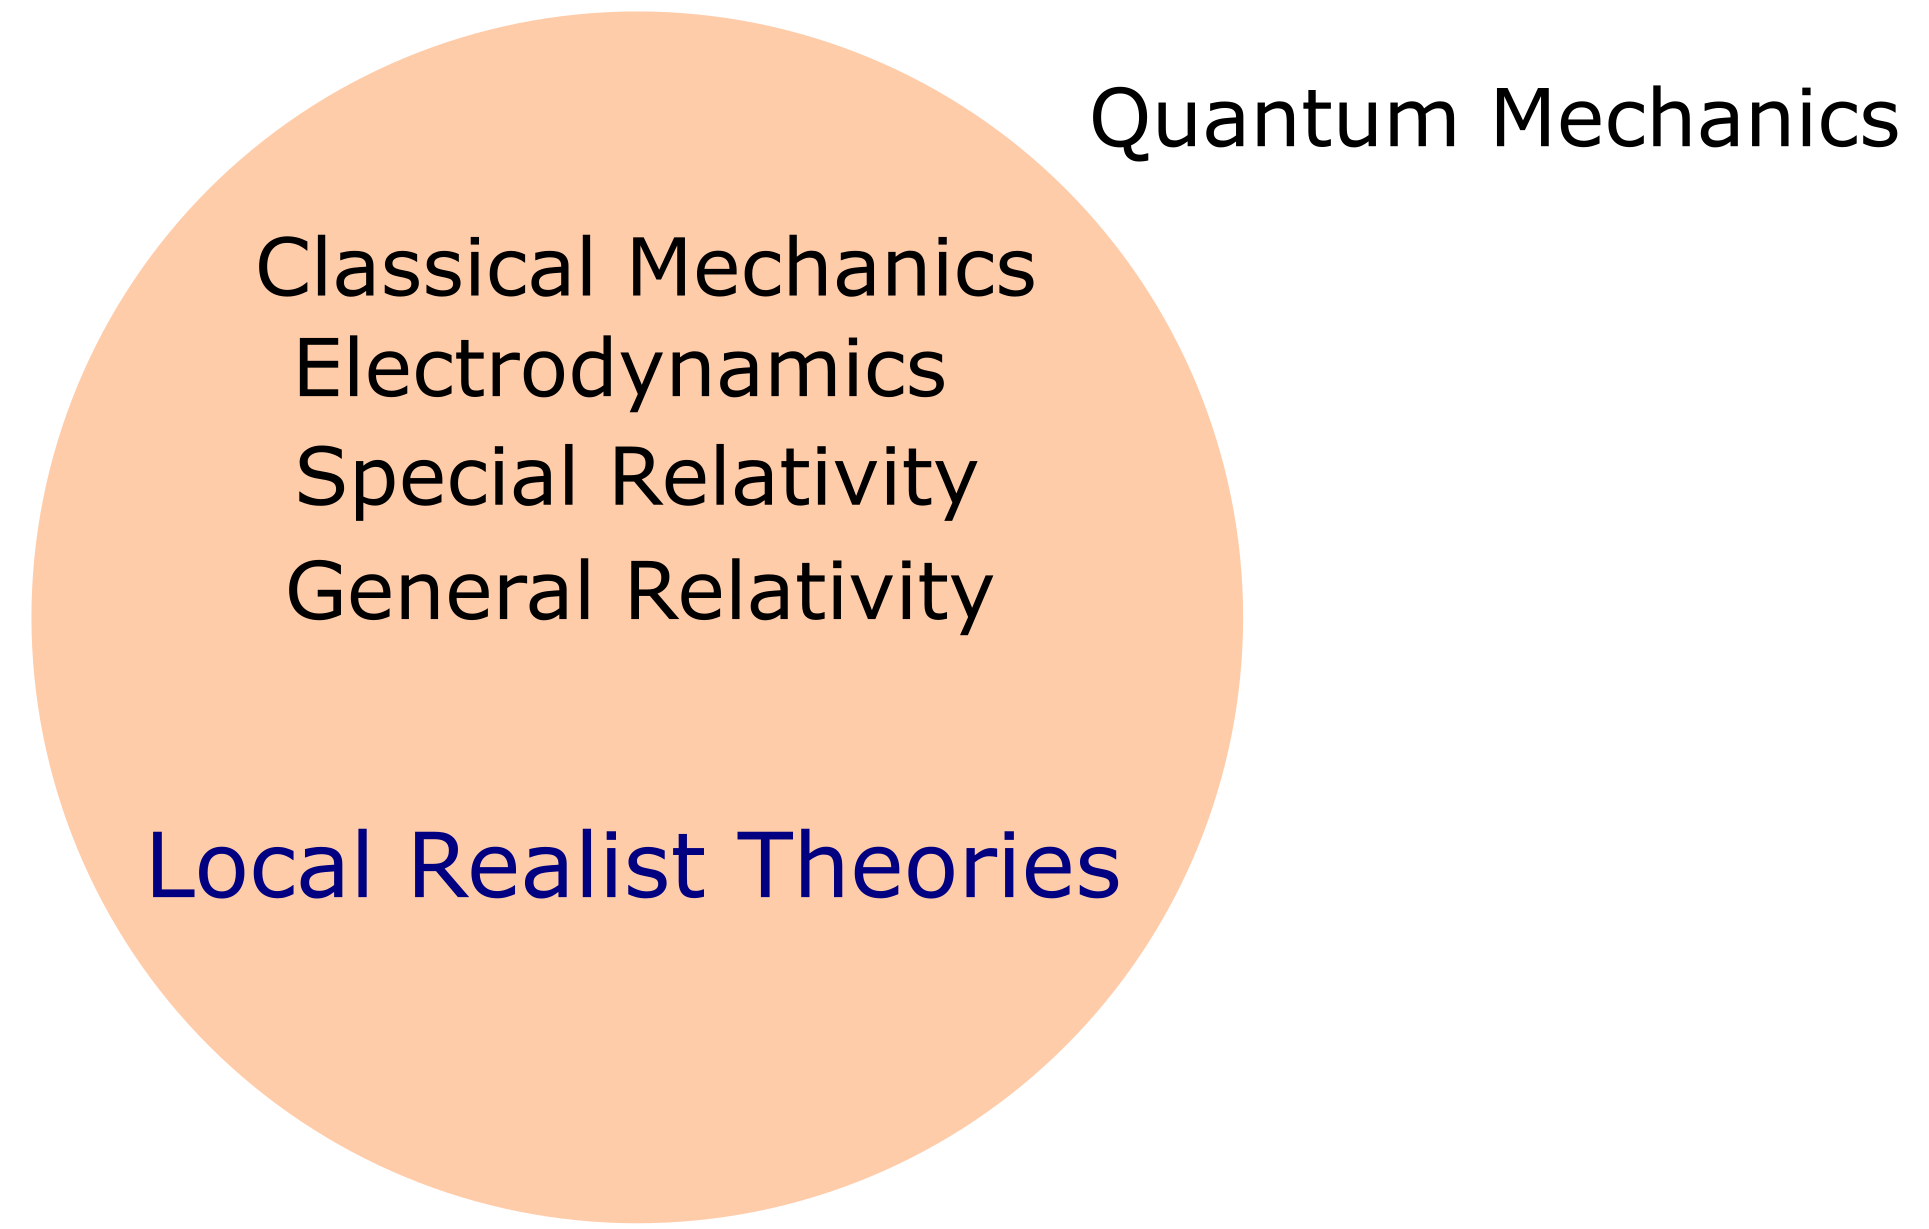
\includegraphics[width=0.62\textwidth]{Images/Local_Realism.png}
    \end{center}
    \begin{block}{Definitions}
        \begin{itemize}
            \item \bf{Realism:} \textnormal{Physical properties are defined prior to and independent of measurement.}
            \item \bf{Local:} \textnormal{Physical influences cannot propagate faster than the speed of light.}
        \end{itemize}
    \end{block}
\end{frame}

\begin{frame}\frametitle{Einstein-Podolsky-Rosen Paradox}
    \begin{center}
        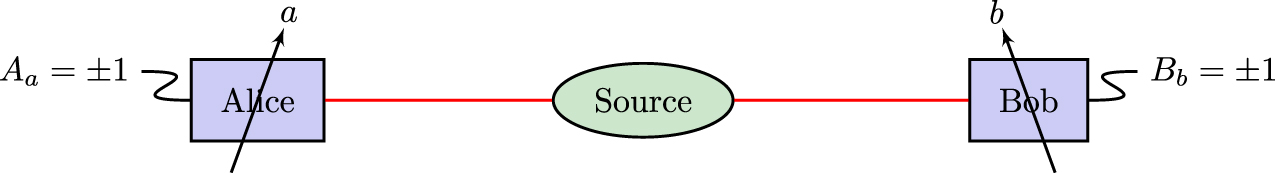
\includegraphics[width=0.9\textwidth]{Images/EPR.jpg}

        \cite{Larsson2014a}
    \end{center}
    \begin{itemize}
        \item A measurement preformed by Alice with settings $a$ affects the result of the measurement 
            preformed by Bob with settings $b$
    \end{itemize}

    \begin{block}{In 1935 EPR write:}
        "This makes the reality of P and Q depend upon the process of measurement carried out on the first system, 
        which does, not disturb the second system in any way. No reasonable definition of reality could be expected 
        to permit this."
        \cite{Brassard2010}
    \end{block}
\end{frame}

\begin{frame}\frametitle{Bell's Inequality}
    EPR proposed the existence of \emph{local hidden variables} to resolve the paradox. In 1971 Bell proposed a 
    statical consequence of these variables ($\lambda\in\Lambda$) through expectation values of an experiment
    $$E(A) = \int_{\Lambda}A(\lambda)\rho(\lambda)d\lambda$$
\end{frame}

\begin{frame}\frametitle{Bell's Inequality}
    Enforcing the condition of local realism Bell used the following assumptions
    \begin{block}{Realism}
        $$A(a,b,\lambda)\qquad B(a,b,\lambda)$$
        Random variables $A$ and $B$ represent measurements and depend on Alice's local 
        settings ($a$), Bob's local settings ($b$), and hidden variable ($\lambda$).
    \end{block}
    \begin{block}{Locality}
            $$A_i(\lambda) \equiv A(a_i,b_1,\lambda) = A(a_i,b_2,\lambda)$$
            $$B_i(\lambda) \equiv B(a_1,b_i,\lambda) = B(a_2,b_i,\lambda)$$
        Measurement outcomes are independent of the remote setting
    \end{block}
    to find the inequality
    $$\left|E(A_2B_1) - E(A_2B_2)\right| \le 1 + E(A_1B_2)$$
\end{frame}

\begin{frame}{Clauser, Horne, Shimony, Holt (CHSH) Inequality}
    CHSH generalized the Bell inequality to by removing the assumption of perfect anticorrelation ($A_i = -B_i$) and
    lessing the outcome restriction to $|A_i|\le1$ and $|B_i|\le1$. The resulting inequality 
    $$\left|E(A_1B_1) + E(A_1B_2)\right| + \left|E(A_2B_1) - E(A_2B_2)\right| \le 2$$
    is experimentally realizable.
\end{frame}

\begin{frame}{Locality (Freedom of Choice) Loophole}
    \begin{center}
    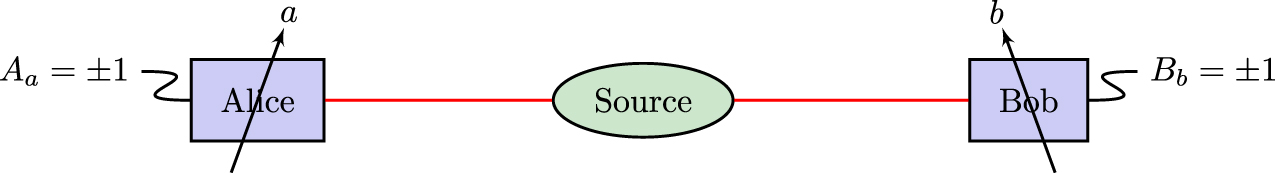
\includegraphics[width=0.9\textwidth]{Images/EPR.jpg}

    \cite{Larsson2014a}
    \end{center}

    In order to prove non-locality the experiment must be designed such that the measurement parameters $a$ and $b$
    are set is such a way that there is no possibility of communication. This achieved by
    \begin{itemize}
        \item Selecting $a$ and $b$ within a fast enough time interval so that Alice and Bob are spacelike separated
        \item Randomizing $a$ and $b$ so that there is no "memory" effecting the measurement
    \end{itemize}
    \begin{block}{Loophole}
        There could still be an event in the intersection of the past light cones of $a$ and $b$ that could cause $a$ and
        $b$ to "know" about each other.
    \end{block}
\end{frame}

\begin{frame}{Dealing with the Loophole: Stars!}
    \begin{center}
    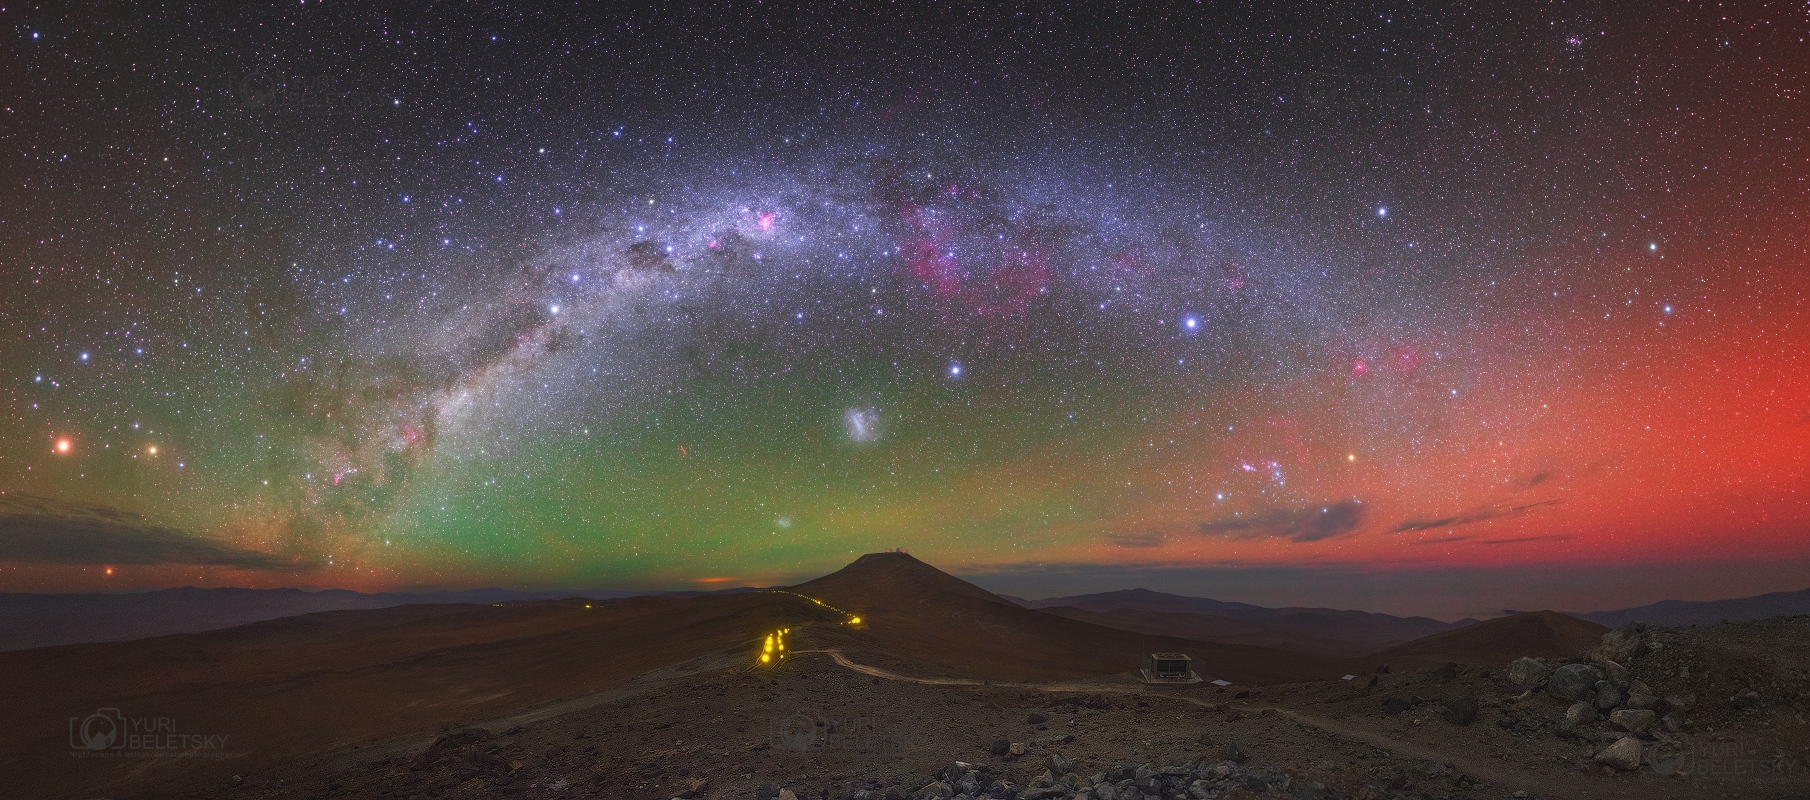
\includegraphics[width=1.0\textwidth]{Images/Milky_way.jpg}
    \end{center}
    Using the wavelength of light from stars in excess of 500 light years away from earth to set the measurement parameters.

\end{frame}

\begin{frame}\frametitle{}
    \centering
    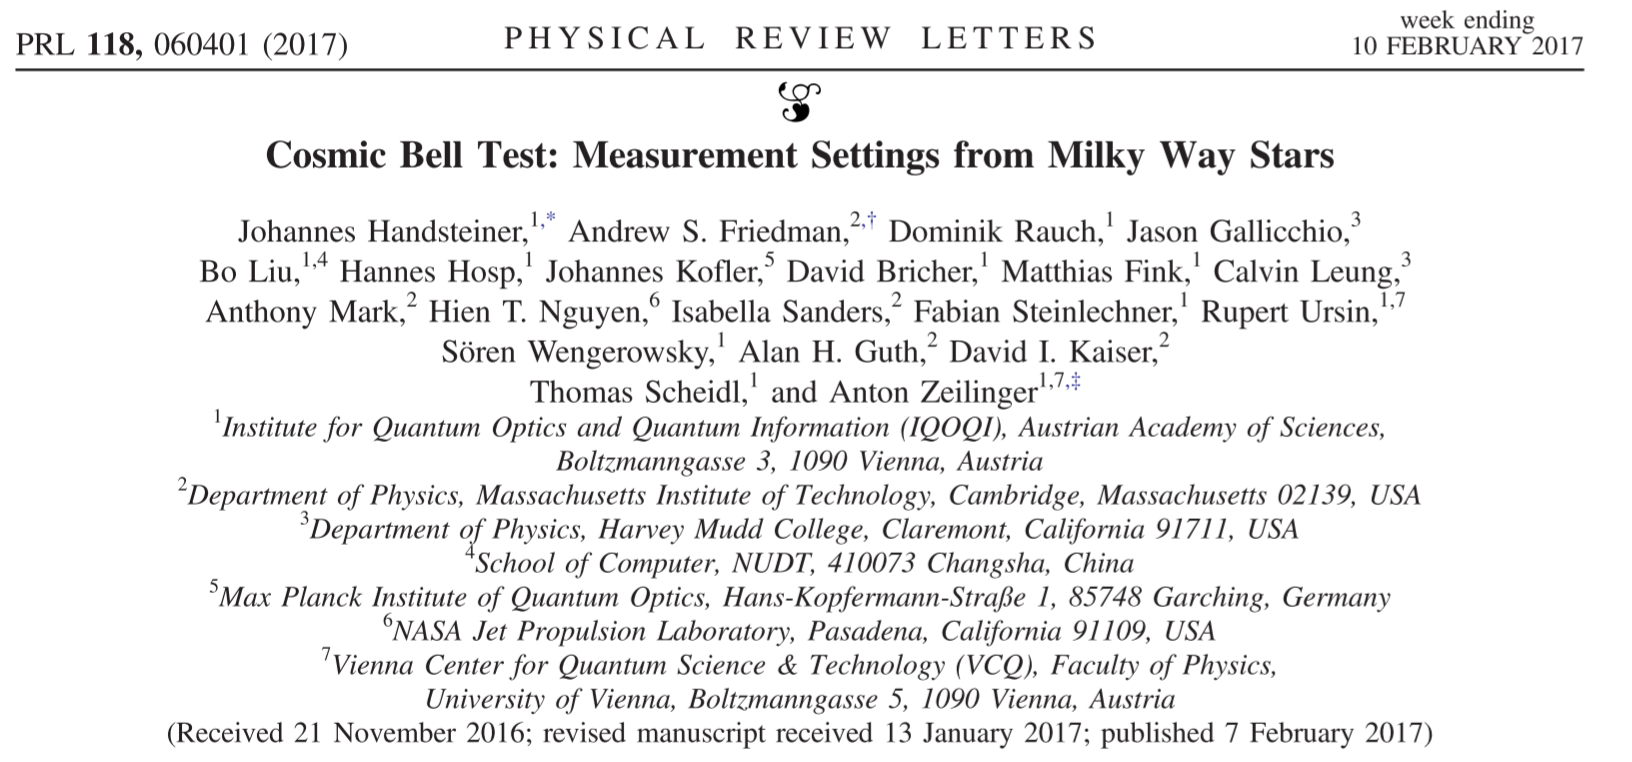
\includegraphics[width=1.0\textwidth]{Images/Paper_Title.png}
\end{frame}

\begin{frame}\frametitle{Experimental Setup}
    \centering
    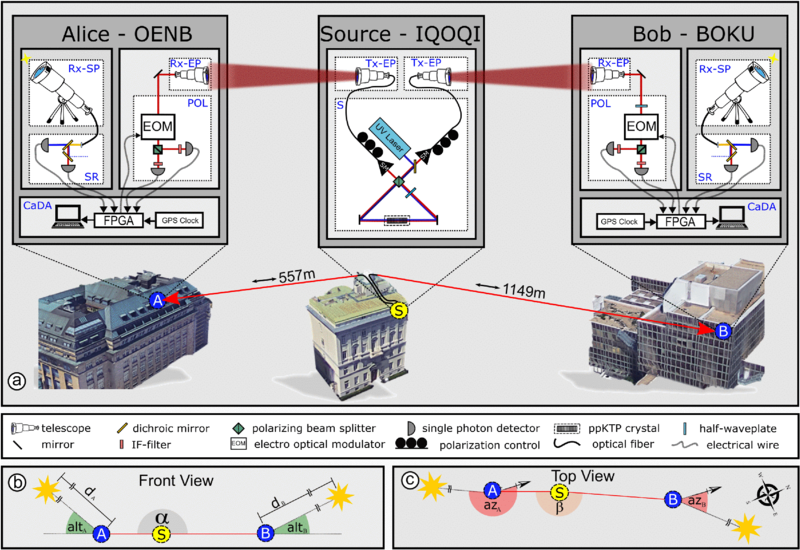
\includegraphics[width=0.88\textwidth]{Images/Exp_Setup.png}

    \cite{Handsteiner2016}
\end{frame}

\begin{frame}\frametitle{Sagnac Interferometer Entangled Photon Generator}
    \centering
    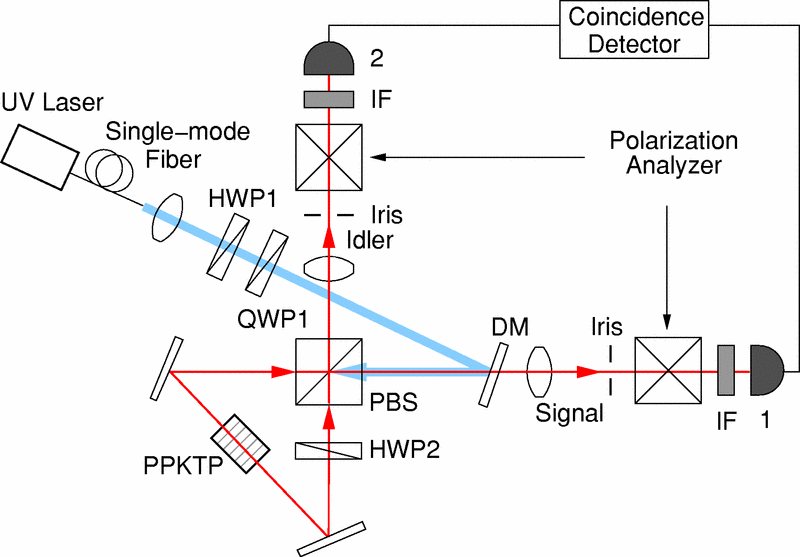
\includegraphics[width=0.8\textwidth]{Images/Sagnac.png}

    \cite{Kim2006}
\end{frame}

\begin{frame}\frametitle{Experimental Space-Time Diagram}
    \centering
    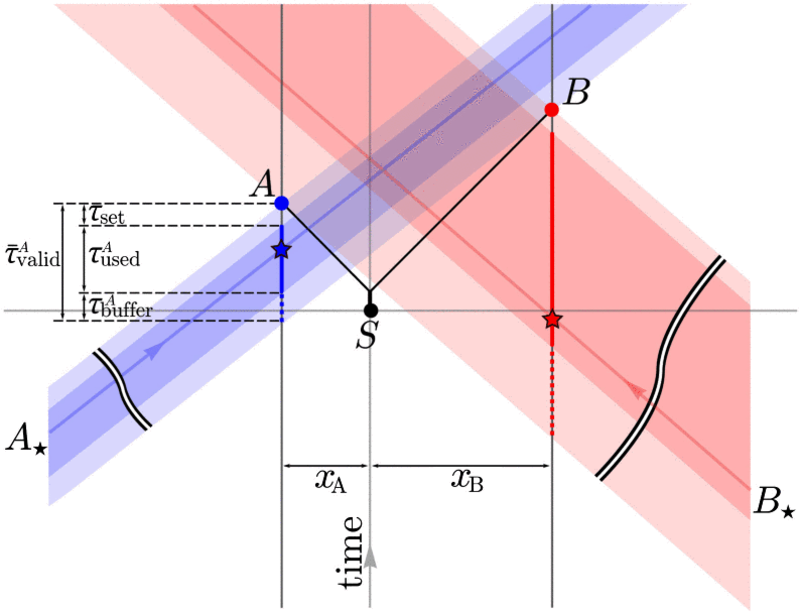
\includegraphics[width=0.75\textwidth]{Images/Light_Lines.png}

    \cite{Handsteiner2016}
\end{frame}

\begin{frame}\frametitle{Experimental Past Light Cones}
    \centering
    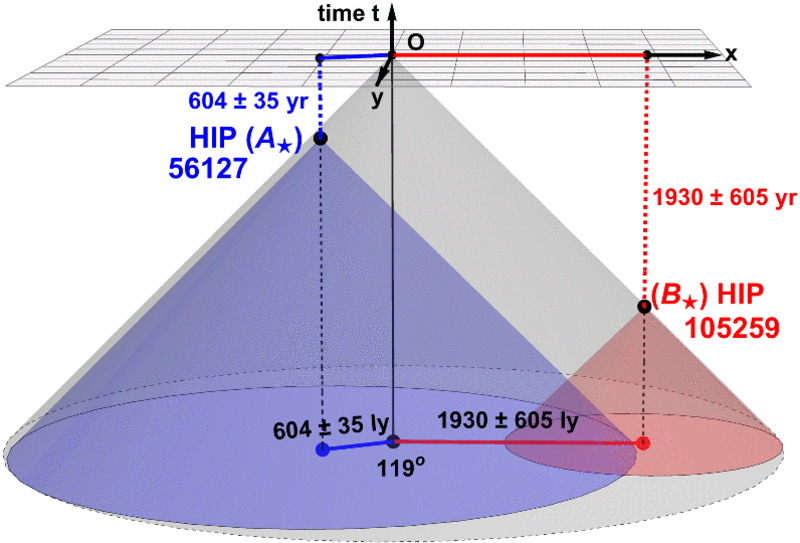
\includegraphics[width=0.8\textwidth]{Images/Light_Cones.png}

    \cite{Handsteiner2016}
\end{frame}

\begin{frame}\frametitle{Results}
    $$\left|E(A_1B_1) + E(A_1B_2)\right| + \left|E(A_2B_1) - E(A_2B_2)\right| \le 2$$
    \centering
    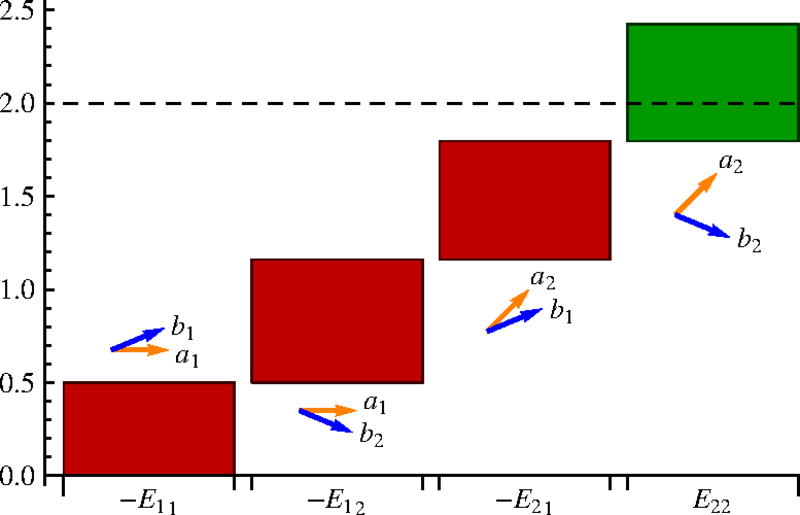
\includegraphics[width=0.8\textwidth]{Images/Corr.png}

    \cite{Handsteiner2016}
\end{frame}

\begin{frame}\frametitle{Results}
    \begin{center}
    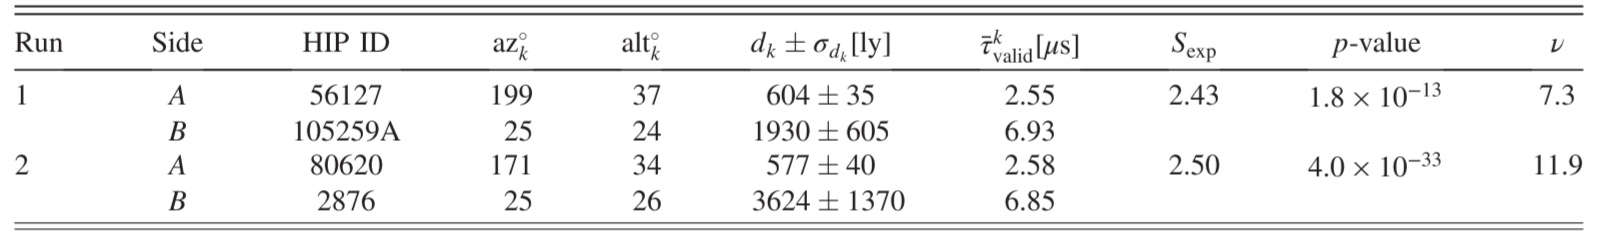
\includegraphics[width=1.0\textwidth]{Images/Results_Table.png}

    \cite{Handsteiner2016}
    \end{center}

    Over two runs each using a different pair of stars they found a violation of the CHSH inequality with a 
    statistical significance bound by at least 7.31 and 11.93 standard deviations for runs 1 and 2 respectively.
\end{frame}

\begin{frame}\frametitle{Conclusion}
    \begin{itemize}
        \item This result forces any local realist model to have acted no more recently
            than $604\pm35$ and $577\pm40$ years ago
        \item And any common cause event must originate from the intersected past light cones at $2409\pm598$ and
            $4040\pm1363$ years ago.
        \item This dramatically limits the space-time region in which hidden variables can remain relevant.
    \end{itemize}
    \begin{block}{}
        "Therefore, any hidden variable mechanism exploiting the freedom of choice loophole would need to have 
        been enacted prior to Gutenberg's invention of the printing press, which itself predates the publication of 
        Newton's Principia by two and a half centuries." \cite{Handsteiner2016}
    \end{block}
\end{frame}

\begin{frame}{Further Reading}
    \tiny
    \bibliographystyle{abbrvnat}
    \bibliography{References}
\end{frame}
\end{document}

